\documentclass[11pt,letterpaper]{article}

\usepackage[left=.5in,right=.5in,top=.75in,bottom=.75in]{geometry}
\usepackage{amsmath,amssymb,bm}
\usepackage{graphicx}
\usepackage{float}
\usepackage{caption}
\usepackage[colorlinks=true,linkcolor=blue,citecolor=blue,urlcolor=blue]{hyperref}

\setlength{\parindent}{0pt}
\setlength{\parskip}{6pt plus 2pt minus 1pt}
\setcounter{secnumdepth}{0}

\captionsetup{font=small,skip=4pt}

\begin{document}

\begin{center}
{\Large\bfseries Approximating Heavy-Tailed Priors With Normal Mixtures \par}
\vspace{0.4em}
{\large A. Demetri Pananos \qquad Tyler Buffington\par}
\vspace{0.15em}
{\footnotesize Datadog Inc. \qquad Datadog Inc.\par}
\end{center}

\vspace{-1.25em}

\subsubsection{Introduction}\label{introduction}

Consider the Bayesian model

\begin{equation}\label{eq-conjugate}
\begin{aligned}
\hat \theta \mid \theta &\sim \operatorname{Normal}(\theta, s^2), \\
\theta &\sim g(\theta).
\end{aligned}
\end{equation}

Here, $\theta$ is the true treatment effect, $\hat \theta$ is its estimate, $s$
is the associated standard error, and $g(\theta)$ is the prior
distribution.  We assume, as is common in A/B testing, that the distribution of $\hat \theta$ conditional on $\theta$ is justified via the Central Limit Theorem and that $s$ is estimated with enough precision to be treated as if known perfectly. Under these assumptions, and given that the
likelihood in (\ref{eq-conjugate}) is normal, it is common for A/B testing platforms to
use a normal prior with variance $\tau^2$ and mean $\mu$, yielding the
conjugate normal model, wherein the posterior is also
normal with variance $\tilde \tau^{2} = (1/s^2 + 1/\tau^2)^{-1}$ and
mean $\tilde \mu = \tilde \tau^{2}(\hat\theta/s^2 + \mu/\tau^2)$. Posterior
quantities (e.g. probabilities, credible intervals, etc.)
are therefore available using only standard normal distribution functions.
Using the conjugate normal model is hence an attractive option because doing so means Bayesian inference
can be scaled to millions of users and implemented across languages and
frameworks without using numerical methods or probabilistic
programming/sampling.

Despite its appeal, the normal prior can be a limiting choice for modeling
treatment effect distributions in practice. Azevedo et al. (2020)
report that noise-adjusted treatment effects for several Bing metrics are heavy-tailed,
and instead fit a Student's $t$ prior for $g(\theta)$ using maximum likelihood. We have observed similar evidence in our own experimentation platform: even after accounting for sampling variation, the empirical distribution of treatment effects exhibits heavy tails. Consistent with this observation, customers who use
empirically informed normal priors occasionally observe extreme outlier effects
with high precision that are nearly impossible under the posterior predictive
distribution. In these cases, those customers have expressed skepticism toward
the resulting shrinkage of the treatment effect, therefore providing indirect evidence of the 
heavy tailed nature of treatment effects. Evidence from Azevedo et al. and our data motivates our interest
in supporting heavy-tailed $g(\theta)$ in (\ref{eq-conjugate}),
but doing so would mean losing an analytical posterior and would generally
require numerical methods.

In this paper, we describe an approach to inference for
(\ref{eq-conjugate}) that we currently use in our experimentation platform and that retains much of the analytical convenience of the conjugate normal model while allowing for heavy-tailed priors. The
main idea is to approximate a target prior distribution by a finite
mixture of normal distributions, so that posterior inference reduces to a
sequence of weighted conjugate normal updates. This strategy is related to
Dalal and Hall (1983), who showed that mixtures of conjugate priors remain
analytically tractable and have desirable convergence properties
which extend to the posterior under suitable conditions. We use quadratic programming to determine the mixture weights. The resulting approximation yields fast posterior
computation for models that would otherwise require numerical integration
or sampling, making it suitable for large-scale experimentation platforms.
Although we use a Student's $t$ distribution as a motivating example
because it is a canonical heavy-tailed prior and has been proposed for
A/B-testing treatment effects by Azevedo et al. (2020), the same strategy
applies to other prior distributions that encode different beliefs about
treatment effects.  

\subsubsection{Methods \& Results}\label{methods-results}

Let $\varphi(x; \mu, \tau)$ denote the density of a normal random variable
with mean $\mu$ and standard deviation $\tau$, and consider the model in
(\ref{eq-conjugate}) in which the prior density for $\theta$ is given by a
$K$-component mixture of normals, each with weight $0 < \pi_k < 1$, 

$$
g(\theta) = \sum_{k=1}^K \pi_k \varphi(\theta;\mu_k,\tau_k),
\qquad
\sum_{k=1}^K \pi_k = 1.
$$

The posterior of $\theta$ under this choice of prior is also a mixture of
normals, and can be written down analytically as a weighted
average of conjugate updates to each component

$$
\Pr(\theta \mid \hat\theta)
=
\sum_{k=1}^K w_k \varphi(\theta;\tilde\mu_k,\tilde\tau_k),
$$

where

$$
\tilde\tau_k^2 = \left(\frac{1}{s^2} + \frac{1}{\tau_k^2}\right)^{-1}, \qquad
\tilde\mu_k = \tilde\tau_k^2 \left(\frac{\hat\theta}{s^2} + \frac{\mu_k}{\tau_k^2}\right), \qquad
w_k =
\frac{\pi_k\,\varphi\!\left(\hat\theta; \mu_k, \sqrt{s^2+\tau_k^2}\right)}
{\sum_{j=1}^K \pi_j\,\varphi\!\left(\hat\theta; \mu_j, \sqrt{s^2+\tau_j^2}\right)}.
$$

Our approach approximates an arbitrary heavy-tailed prior, $h(\theta)$, by fitting a
mixture of normals with a fixed set of means and standard deviations,
$\{(\mu_k,\tau_k)\}_{k=1}^K$, and estimating only the mixture weights
$\boldsymbol{\pi}=(\pi_1,\ldots,\pi_K)^\top$. We choose the weights by
minimizing Pearson's chi-square divergence from the mixture $g$ to the
target $h$. This target-weighted squared relative error controls the total-variation distance between the approximate and target priors, and Dalal and Hall (1983) show that convergence of the priors in total variation yields convergence of the corresponding posteriors. This choice of divergence is especially
attractive because it admits a quadratic representation for fixed $(\mu_k,\tau_k)$, 
namely

$$
\begin{aligned}
\chi^2(g\Vert h)
&=
\int
\frac{\{g(\theta)-h(\theta)\}^2}{h(\theta)}\,d\theta
=\boldsymbol{\pi}^{\top}C\boldsymbol{\pi}-1,\\
C_{jk}
&=
\int
\frac{\varphi(\theta;\mu_j,\tau_j)\varphi(\theta;\mu_k,\tau_k)}
{h(\theta)}\,d\theta,\\
\widehat{\boldsymbol{\pi}}
&=
\underset{\boldsymbol{\pi}\geq0,\ \mathbf{1}^{\top}\boldsymbol{\pi}=1}
{\operatorname{arg\,min}}
\left\{
\frac{1}{2}\boldsymbol{\pi}^{\top}C\boldsymbol{\pi}
+\frac{\lambda}{2}\lVert\boldsymbol{\pi}\rVert_2^2
\right\}.
\end{aligned}
$$

When its entries are finite, $C$ is a positive-semidefinite Gram matrix,
so estimating the mixture weights reduces to a convex quadratic program.
Consequently, the weights can be computed using standard quadratic
programming algorithms. We add a small ridge penalty,
$\lambda=1\times10^{-8}$, to make the objective strictly convex. Once obtained, the weights can be stored and used for multiple analyses.

To demonstrate the approach, we approximate a Student's $t$ prior with 3
degrees of freedom, location $0$, and scale $0.05$. Although the Student's
$t$ distribution admits a known scale-mixture-of-normals representation,
and so our approach is not strictly needed for this case, it provides a
useful benchmark. Because the target prior is symmetric about zero, we use a mixture of
$K=80$ zero-mean normals, $\varphi(\theta;0,\tau_k)$, with
$\tau_k$ logarithmically spaced from $0.002$ to $1.5$. The resulting fit,
plotted over the range from the $0.01$th to the $99.99$th percentile of
the target prior, is shown in Figure~\ref{fig-shrinkage}. The close
agreement on the log scale shows that the normal mixture closely
approximates the center and tails of the distribution over the indicated range.
The mixture also closely reproduces the
shrinkage behavior of the heavy-tailed prior over the range of observed
z-values: the posterior mean divided by the observed standard error,
$\tilde z = \operatorname{E}(\theta \mid \hat\theta)/s$, is shrunk
strongly near zero but much less for large observed $z = \hat\theta/s$.
Finally, simulation-based calibration over $10{,}000$ datasets
generated under the exact target prior and analyzed using the mixture
shows no evidence of systematic miscalibration, suggesting small posterior
distortion in aggregate from replacing the target prior in (\ref{eq-conjugate}) with its
normal-mixture approximation.


\subsubsection{Limitations \& Discussion}\label{limitations-discussion}

Finite normal mixtures provide a practical way to use heavy-tailed priors in (\ref{eq-conjugate}) while retaining much of the analytical convenience of conjugate Bayesian inference. Once the mixture weights are estimated, posterior densities, means, probabilities, and credible intervals can be computed using inexpensive finite-mixture calculations. In our example, the approximation closely reproduces the target density, its implied nonlinear shrinkage, and its aggregate calibration over the range examined.

The approach has one principal limitation. A finite normal mixture is ultimately not heavy-tailed: its asymptotic behavior is determined by its widest normal component, which remains normal. The method should therefore be viewed as an approximation to a heavy-tailed prior over a prespecified operational range, rather than as an exact representation of its asymptotic tail behavior.

Despite this limitation, the method provides a computationally efficient bridge between conjugate normal models and richer prior distributions. It is particularly attractive for large-scale experimentation platforms, where a target prior may be estimated or elicited once, approximated offline through convex optimization, and then reused for repeated posterior inference. Although we demonstrate the method using a Student's $t$ prior, the same approach can be applied to other target priors that encode alternative beliefs about the distribution of treatment effects.



\begin{thebibliography}{9}

\bibitem{azevedo2020}
Azevedo, Eduardo M., Alex Deng, Jos\'e Luis Montiel Olea, Justin Rao,
and E. Glen Weyl. 2020. ``A/B Testing with Fat Tails.''
\emph{Journal of Political Economy} 128 (12): 4614--4672.


\bibitem{dalal1983}
Dalal, S. R., and W. J. Hall. 1983.
``Approximating Priors by Mixtures of Natural Conjugate Priors.''
\emph{Journal of the Royal Statistical Society: Series B
(Methodological)} 45 (2): 278--286.


\end{thebibliography}

\begin{figure}[H]
\centering
\IfFileExists{assets/figure_1.png}{
  \makebox[\linewidth][c]{%
    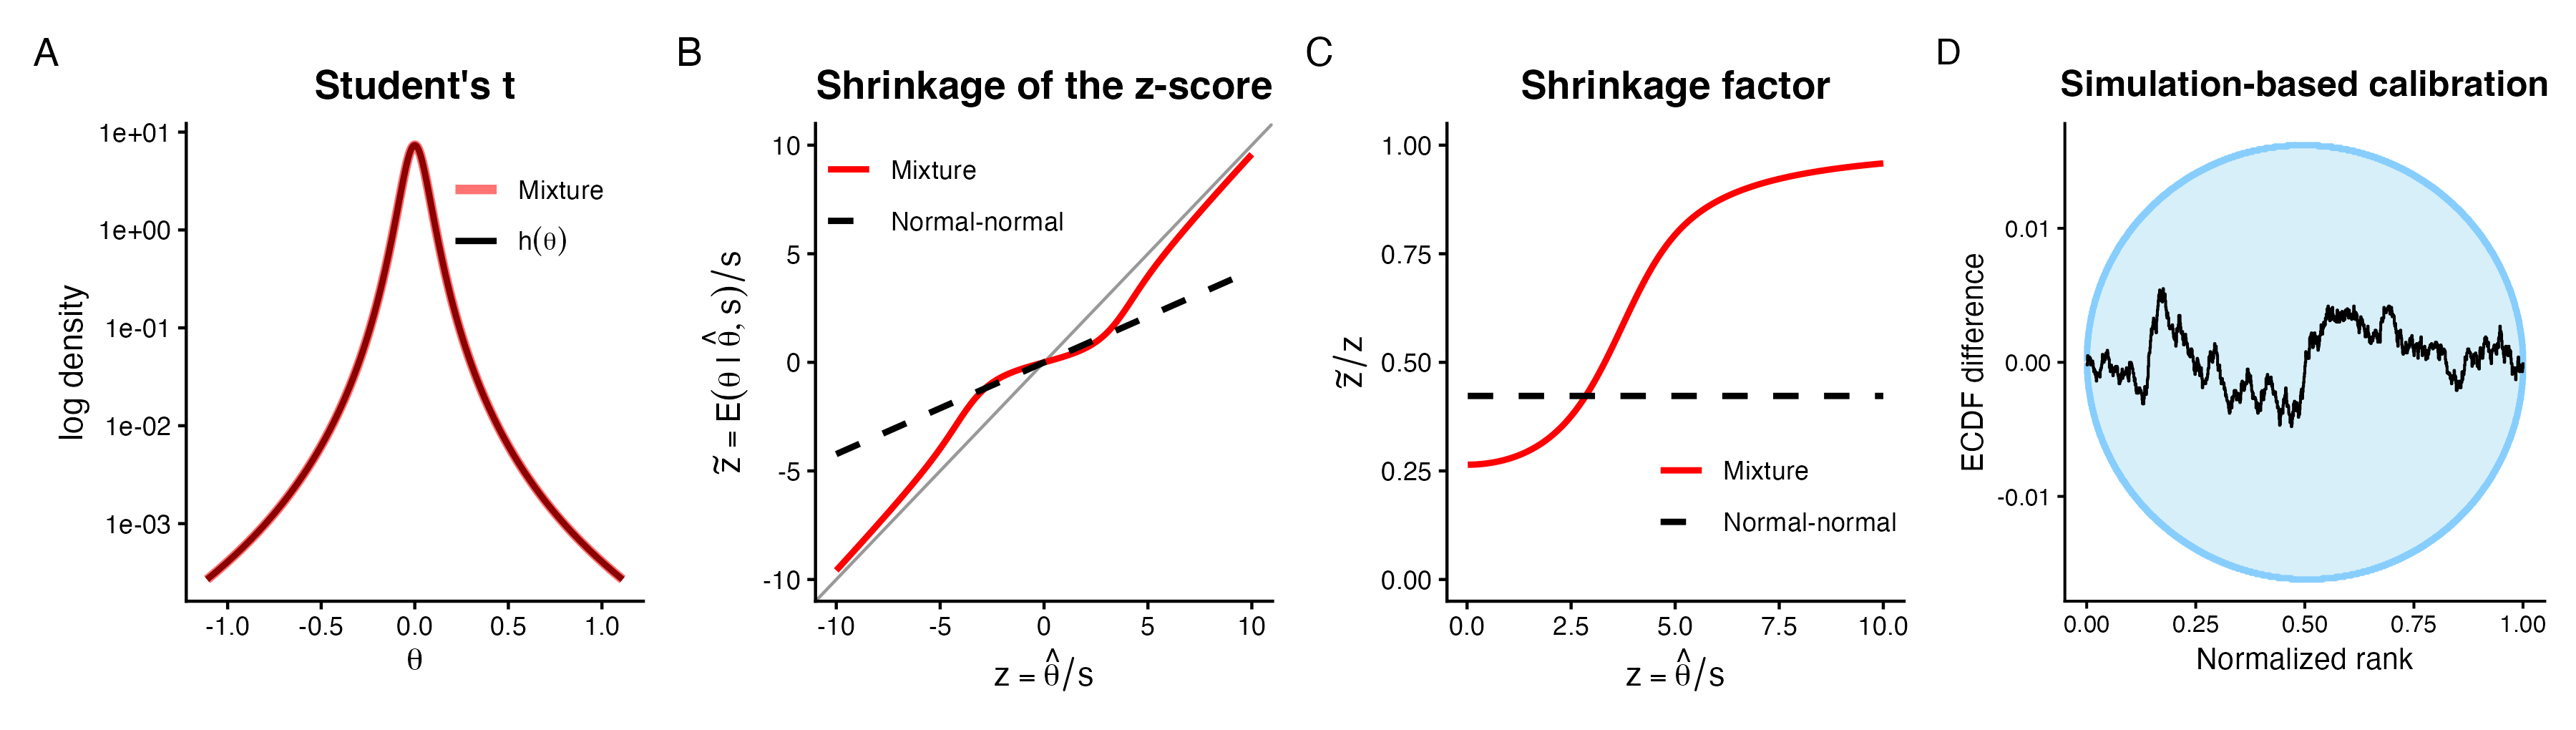
\includegraphics[width=1.08\linewidth,keepaspectratio]{assets/figure_1.png}%
  }
}{
  \fbox{\parbox{0.9\linewidth}{\centering Figure file \texttt{assets/figure_1.png} not found.}}
}

\caption{\label{fig-shrinkage}
Normal-mixture approximation and implied shrinkage for a Student's $t$
prior. (A) Log density of the target Student's $t$ prior, with 3 degrees of
freedom, location $0$, and scale $0.05$, and its normal-mixture approximation.
(B) Posterior mean divided by observed standard error, $\tilde z =
\operatorname{E}(\theta \mid \hat\theta)/s$, as a function of $z =
\hat\theta/s$ for $s = 0.1$. The conjugate normal model produces constant
proportional shrinkage, shown by the black dashed line, while the mixture
prior adaptively shrinks small effects more than large effects. The grey line
is the identity. (C) The same behavior expressed as the shrinkage factor
$\tilde z / z$. (D) Simulation-based calibration (SBC) over 10,000 datasets generated under the target Student’s $t$ prior. The empirical distribution of SBC ranks remains close to the uniform distribution expected under perfect calibration and within the reference envelope, indicating no detectable systematic miscalibration from the normal-mixture approximation.}
\end{figure}

\end{document}